\item\problemnumber{GT R}{4}{1}{-}{.}
Consider the insertion of items with the following keys (in the given order)
into an initially empty AVL tree: $30,40,24,58,48,26,11,13$. Draw the final tree
that results.\\[12pt]
\ifanswers
\textcolor{blue}{
\textbf{Answer:}\\[6pt]
Answer goes here\parend
Here is the result of adding the keys in the given order into a regular binary
search tree:\\[12pt]
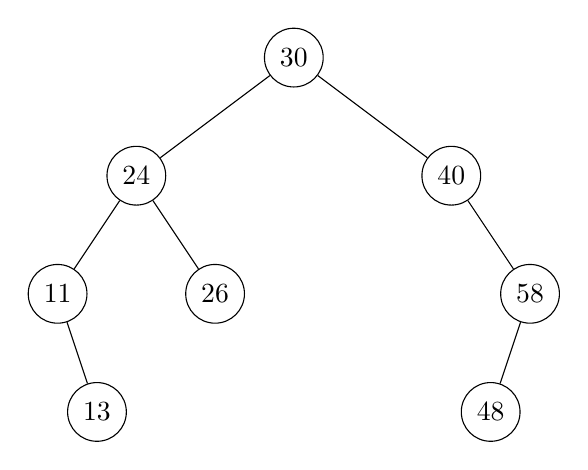
\begin{tikzpicture}
    \node[circle,draw] at (4,4.5) (n1) {$30$};
    \node[circle,draw] at (6,3) (n2) {$40$};
    \node[circle,draw] at (2,3) (n3) {$24$};
    \node[circle,draw] at (7,1.5) (n4) {$58$};
    \node[circle,draw] at (6.5,0) (n5) {$48$};
    \node[circle,draw] at (3,1.5) (n6) {$26$};
    \node[circle,draw] at (1,1.5) (n7) {$11$};
    \node[circle,draw] at (1.5,0) (n8) {$13$};
    \draw[-] (n1)--(n2);
    \draw[-] (n1)--(n3);
    \draw[-] (n3)--(n6);
    \draw[-] (n3)--(n7);
    \draw[-] (n2)--(n4);
    \draw[-] (n7)--(n8);
    \draw[-] (n4)--(n5);
\end{tikzpicture}
\vskip12pt
Note: This is just to provide an example of drawing a tree in \LaTeX. Please
replace it with your answer.
}
\newpage
\fi
